\uuid{izYW}
\exo7id{5428}
\titre{exo7 5428}
\auteur{exo7}
\organisation{exo7}
\datecreate{2010-07-06}
\isIndication{false}
\isCorrection{true}
\chapitre{Développement limité}
\sousChapitre{Calculs}

\contenu{
\texte{
Soit $0<a<b$. Etude complète de la fonction $f(x)=\left(\frac{a^x+b^x}{2}\right)^{1/x}$.
}
\reponse{
Puisque $a>0$, $b>0$ et que pour tout réel $x$, $\frac{a^x+b^x}{2}>0$, $f$ est définie sur $\Rr^*$, et pour

\begin{center}
$\forall x\in\Rr^*$, $f(x)=\text{exp}\left(\frac{1}{x}\ln\left(\frac{a^x+b^x}{2}\right)\right)$.
\end{center}
\textbf{Etude en 0}.

\begin{align*}\ensuremath
\ln\left(\frac{a^x+b^x}{2}\right)&=\ln\left(\frac{e^{x\ln a}+e^{x\ln b}}{2}\right)\underset{x\rightarrow0}{=}\ln\left(1+x\left(\frac{1}{2}\ln a+\frac{1}{2}\ln b\right)+x^2\left(\frac{1}{4}\ln^2a+\frac{1}{4}\ln^2b\right)+o(x^2)\right)\\
 &=\ln\left(1+x\ln\left(\sqrt{ab}\right)+x^2\frac{\ln^2a+\ln^2b}{4}+o(x^2)\right)=x\ln\left(\sqrt{ab}\right)+x^2\frac{\ln^2a+\ln^2b}{4}-\frac{1}{2}(x\ln\sqrt{ab})^2+o(x^2)\\
 &=x\ln\left(\sqrt{ab}\right)+\frac{1}{8}(\ln^2a-2\ln a\ln b+\ln^2b)x^2+o(x^2)=x\ln\left(\sqrt{ab}\right)+x^2\frac{1}{8}\ln^2\left(\frac{a}{b}\right)+o(x^2).
\end{align*}
Enfin,

$$f(x)=\left(\frac{a^x+b^x}{2}\right)^{1/x}=\mbox{exp}(\ln(\sqrt{ab})+\frac{1}{8}\ln^2\frac{a}{b}x+o(x))=\sqrt{ab}(1+\frac{1}{8}x\ln^2\frac{a}{b}+o(x)).$$
Ainsi, $f$ se prolonge par continuité en $0$ en posant $f(0)=\sqrt{ab}$. Le prolongement obtenu est dérivable en $0$ et
$f'(0)=\frac{\sqrt{ab}}{8}\ln^2\frac{a}{b}(>0)$.
\textbf{Etude en} $\bf{+\infty}$.
\begin{align*}\ensuremath
\frac{1}{x}\ln\left(\frac{1}{2}(a^x+b^x)\right)&=\frac{1}{x}\left(\ln(b^x)-\ln2+\ln\left(1+\left(\frac{a}{b}\right)^x\right)\right)
=\frac{1}{x}(x\ln b+o(x))\quad(\mbox{car}\;0<\frac{a}{b}<1)\\
 &=\ln b+o(1).
\end{align*}
et $\lim_{x\rightarrow +\infty}f(x)=b(=\mbox{Max}\{a,b\})$.
\textbf{Etude en} $\bf{-\infty}$. Pour tout réel $x$,

$$f(-x)=\left(\frac{a^{-x}+b^{-x}}{2}\right)^{-1/x}= \left(\frac{a^{x}+b^{x}}{2a^xb^x}\right)^{-1/x}=\frac{ab}{f(x)},$$
et donc,

$$\lim_{x\rightarrow -\infty}f(x)=\lim_{X\rightarrow +\infty}f(-X)=\lim_{X\rightarrow +\infty}\frac{ab}{f(X)}=\frac{ab}{b}=a\quad(=\mbox{Min}\{a,b\}).$$
\textbf{Dérivée et variations}.
$f$ est dérivable sur $]-\infty,0\cup]0,+\infty[$ en vertu de théorèmes généraux (et aussi en $0$ d'après l'étude faite plus haut), et pour $x\neq0$ (puisque $f>0$ sur $\Rr^*$),

$$\frac{f'(x)}{f(x)}=(\ln f)'(x)=\left(\frac{1}{x}\ln\left(\frac{a^x+b^x}{2}\right)\right)'(x)=-\frac{1}{x^2}\ln\left(\frac{a^x+b^x}{2}\right)+\frac{1}{x}
\frac{a^x\ln a+b^x\ln b}{a^x+b^x}.$$
$f'$ a le même signe que $(\ln f)'$ qui, elle-même, a le même signe que la fonction $g$ définie sur $\Rr$ par

$$\forall x\in\Rr,\;g(x)=-\ln\left(\frac{a^x+b^x}{2}\right)+x\frac{a^x\ln a+b^x\ln b}{a^x+b^x}.$$
$g$ est dérivable sur $\Rr$ et, pour $x$ réel,

\begin{align*}\ensuremath
g'(x)&=-\frac{a^x\ln a+b^x\ln b}{a^x+b^x}+\frac{a^x\ln a+b^x\ln b}{a^x+b^x}+x\frac{(a^x\ln^2a+b^x\ln^2b)(a^x+b^x)-(a^x\ln a+b^x\ln b)^2}{(a^x+b^x)^2}\\
 &=x\frac{(ab)^x(\ln a-\ln b)^2}{(a^x+b^x)^2}.
\end{align*}
$g'$ est donc strictement négative sur $]-\infty,0[$ et strictement positive sur $]0,+\infty[$. Par suite, $g$ est strictement décroissante sur $]-\infty,0]$ et strictement croissante sur $[0,+\infty[$. $g'$ admet donc un minimum global strict en $0$ et puisque $g(0)=0$, on en déduit que $g$ est strictement positive sur $\Rr^*$. De même, $f'$ est strictement positive sur $\Rr^*$. En tant compte de l'étude en $0$, on a montré que $f$ est dérivable sur $\Rr$ et que $f'$ est strictement positive sur $\Rr$. $f$ est donc strictement croissante sur $\Rr$.
Le \textbf{graphe de $f$} a l'allure suivante~:

$$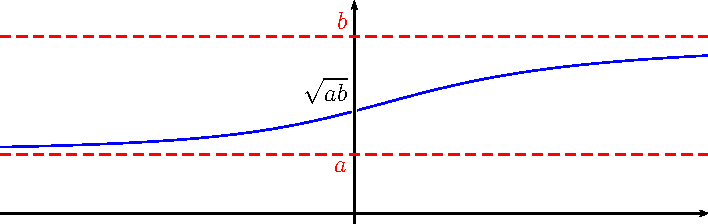
\includegraphics{../images/img005428-1}$$

On peut noter que les inégalités $\lim_{x\rightarrow -\infty}f<f(-1)<f(0)<f(1)<\lim_{x\rightarrow +\infty}f$ fournissent~:

$$a<\frac{1}{\frac{1}{2}(\frac{1}{a}+\frac{1}{b})}<\sqrt{ab}<\frac{a+b}{2}<b.$$
}
}
